\section{JSON Protection Model}
%In this section, we explain our protection model  using a simple JSON document (Fig. \ref{fig:json-example}) and  authorization policies given below.
%\begin{enumerate}
%	\item  \textit{emergency response team} can read all \textit{contact information} (personal phone number, personal email address, work phone number  and work  email address).
%	\item \textit{Manager} can read \textit{work record} but not \textit{confidential work record} (SSN, or salary when greater than 60000).
%	\item \textit{HR} can read  \textit{work record} and \textit{ identifiable personal record} of an employee.
%\end{enumerate}

Our JSON protection model requires following steps to be worked out.


\begin{figure}[t]
	%\vspace{-15pt}
	\centering
	\label{fig:protection-model}
		
	\begin{minipage}{.5\textwidth}
		\centering
		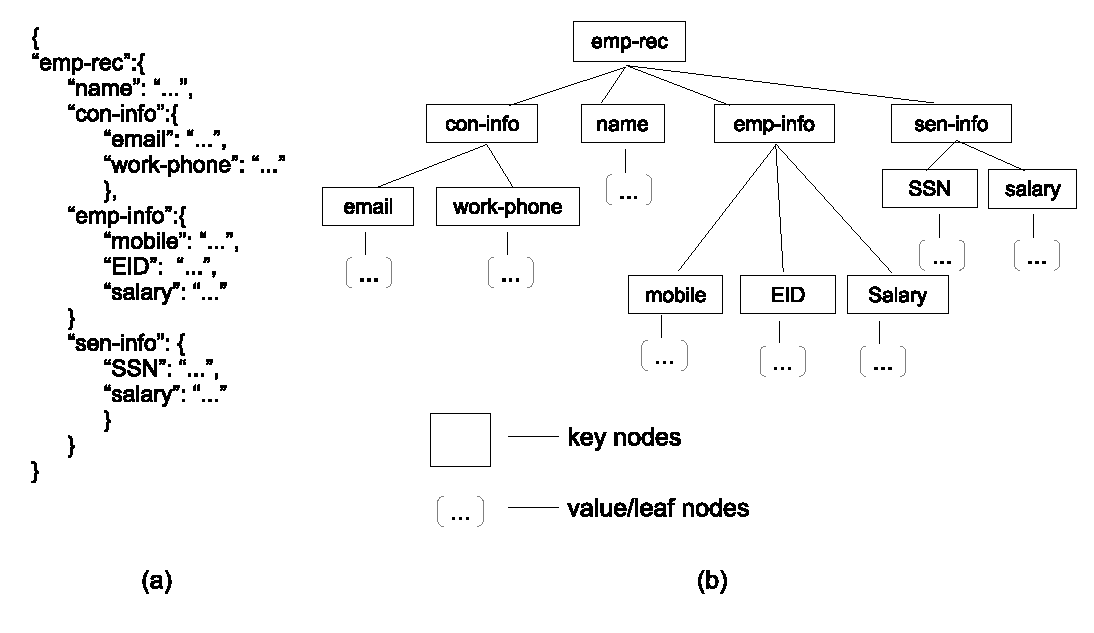
\includegraphics[height=1.1\textwidth]{json-example.eps}
		\label{fig:json-example}
	\end{minipage}%
	\begin{minipage}{.5\textwidth}
			\centering
			\includegraphics[height=0.8\textwidth]{hierarchy.eps}
			%\caption{\indent object label hierarchy, b. user label hierarchy}
			\label{fig:hierarchy}
		\end{minipage}%
\caption{\ref{fig:json-example}A JSON document (visually enhanced) containing an employee information, \ref{fig:hierarchy} object-label and user-label hierarchy}
\end{figure}

\begin{enumerate}
	\item \textbf{Specifying object-label and user-label values.}
	\item \textbf{Configuring policy using specified labels.}
	\item \textbf{Assigning labels on objects and users.}
%	
%	\item \textbf{Labeling JSON Items} We assign  object-label values on JSON items in the JSON document. On the other hand, users are assigned user-label values which are essentially user roles. Object labels, user labels and their hierarchies are shown in Fig. \ref{fig:hierarchy}. 
%	
%	\item \textbf{Configuring LaBAC policy} We use LaBAC policy to specify users associated a user label  can access objects associated with which object-labels. 
	\end{enumerate}
	
\subsection{Specifying labels and configuring policies}	
% Following lists the LaBAC policies for the above requirements  assuming that JSON items and users have been labeled using labels in Fig. \ref{fig:hierarchy}. We discuss actual labeling in the next section.
%	\begin{enumerate}
%		\item (\{emergency response team\},read, \{work contact, personal contact\})
%		\item (\{manager\},read,\{work record, work contact\})
%		\item (\{HR\},read,\{work confidential, work contact, identifiable record\})
%	\end{enumerate}
%
